\documentclass[aps,prc,onecolumn,amsmath,amssymb, preprint, 12pt]{revtex4-1}
\usepackage{graphicx}  % needed for figures
\usepackage{dcolumn}   % needed for some tables
\usepackage{bm}        % for math
\usepackage{verbatim}   % for math
\bibliographystyle{apsrev4-1}
\usepackage{textcomp}
\usepackage{subfigure}
% \usepackage{sidecap} %%caption on side figures

\usepackage{mathptmx} %%use times new roman
%Remove the spacing between paragraphs and have a small paragraph indentation
\setlength{\parskip}{0cm}
\setlength{\parindent}{1em}
%Remove space around section headings.
%\usepackage[compact]{titlesec}
%\titlespacing{\section}{0pt}{2ex}{1ex}
%\titlespacing{\subsection}{0pt}{1ex}{0ex}
%\titlespacing{\subsubsection}{0pt}{0.5ex}{0ex}



\renewcommand{\baselinestretch}{1.5} 

\begin{document}

\pagenumbering{roman}
%%%%%====================================================================================
% % The following information is for internal review, please remove them for submission
% \widetext
% \leftline{Version 01 as of \today}
% \leftline{To be submitted to PAC42 at NSCL}
% \leftline{Comment to {\tt zamora@nscl.msu.edu} by xxx, yyy}
% \centerline{\em  INTERNAL DOCUMENT -- NOT FOR PUBLIC DISTRIBUTION}
%%%%%====================================================================================


%%%%%====================================================================================
\title{  Inclusive Breakup \textit{vs.} Transfer Reactions of ${}^{6}$Li on Light Targets }
%%%%%====================================================================================



%%%%%====================================================================================
%\input author_list.tex       % input author_list 
%%%%%====================================================================================






   
   
\date{\today}

%%%%%====================================================================================
% \begin{abstract}
% Some abstract
% \end{abstract}
%%%%%====================================================================================
% \maketitle




\pagenumbering{arabic}

\section{Experiment}



\begin{figure}[!ht]
\centering
\includegraphics[width=0.9\textwidth]{/home/juan/proyectos/pattpc_14O_alpha/twinsol.eps}
 \caption{\label{setup}  Experimental setup. TWINSOL coupled with the pAT-TPC. A 54\% pure ${}^{17}$F beam at 34.7~MeV was injected into the pAT-TPC. The pAT-TPC was filled with pure ${}^{4}$He gas at 350~Torr. }
 \end{figure}


\section{Preliminary Results}





\begin{figure}[!ht]
\centering
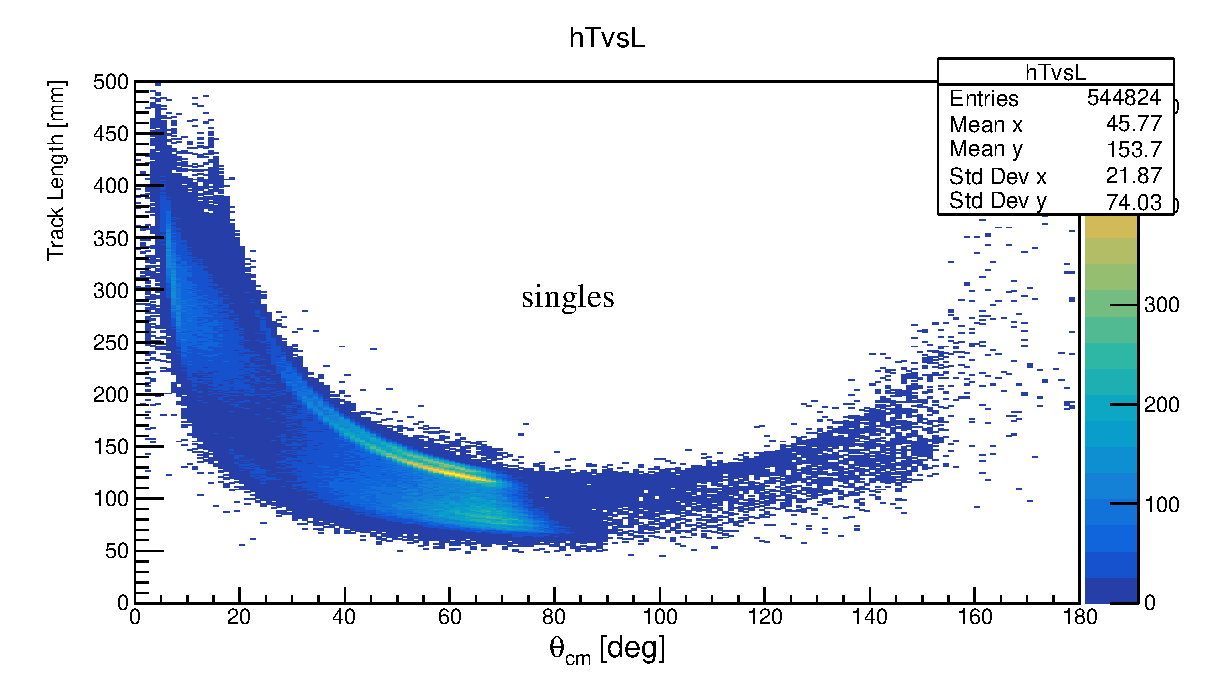
\includegraphics[width=0.49\textwidth]{singles.eps}
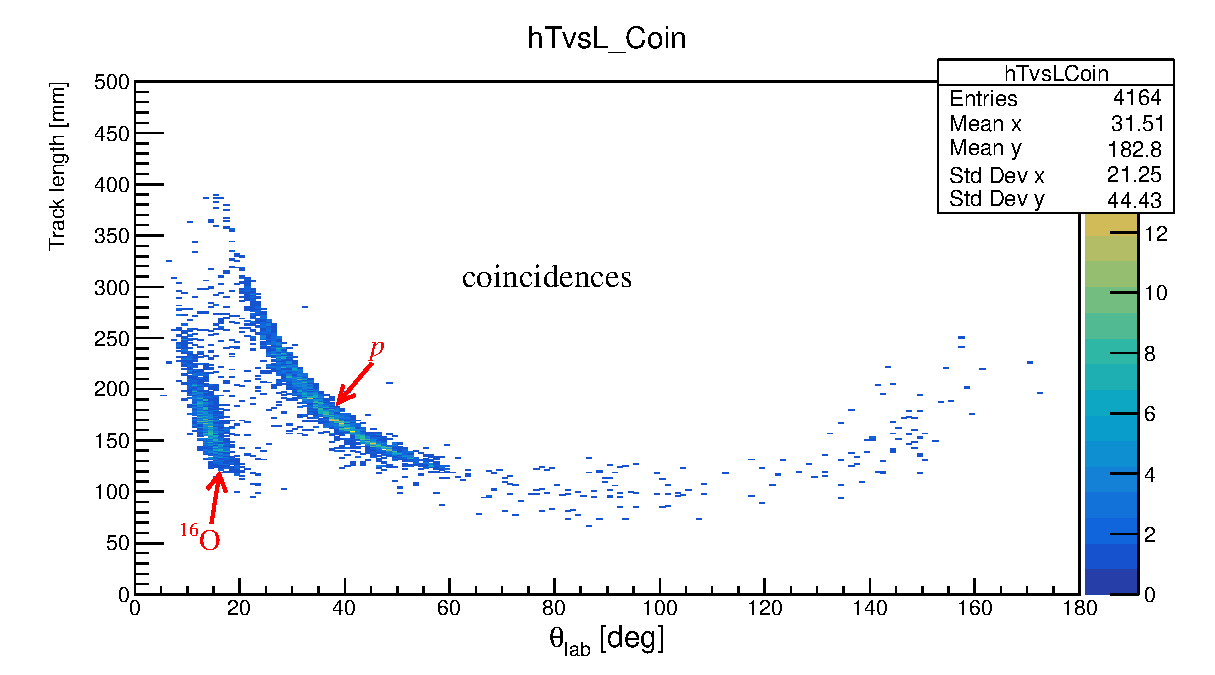
\includegraphics[width=0.49\textwidth]{coin.eps}\\
 \caption{\label{pid}  PID for the scattered particles. The singles spectra is dominated by ${}^{4}$He scattering. Protons and hevy-ion particles can also be selected in coincidence events with only one reaction vertex.  }
 \end{figure}



\begin{figure}[!ht]
\centering
\includegraphics[width=0.49\textwidth]{ad_70.eps}
\includegraphics[width=0.49\textwidth]{ad_80.eps}\\
\includegraphics[width=0.49\textwidth]{ad_90.eps}
\includegraphics[width=0.49\textwidth]{ad_100.eps}\\
\includegraphics[width=0.49\textwidth]{ad_110.eps}
\includegraphics[width=0.49\textwidth]{ad_120.eps}\\
 \caption{\label{proton1}  Proton production (inclusive) and Breakup events in coincidence with ${}^{16}$O particles (exclusive) for different energies. }
 \end{figure}



\begin{figure}[!ht]
\centering
\includegraphics[width=0.49\textwidth]{ad_130.eps}
\includegraphics[width=0.49\textwidth]{ad_140.eps}\\
\includegraphics[width=0.49\textwidth]{ad_150.eps}
\includegraphics[width=0.49\textwidth]{ad_160.eps}\\
\includegraphics[width=0.49\textwidth]{ad_170.eps}
\includegraphics[width=0.49\textwidth]{ad_180.eps}\\
 \caption{\label{proton2}  Same as Fig.~\ref{proton1} but for a different energy range. }
 \end{figure}
 

 
\begin{figure}[!ht]
\centering
\includegraphics[width=0.49\textwidth]{ad_190.eps}
\includegraphics[width=0.49\textwidth]{ad_200.eps}\\
\includegraphics[width=0.49\textwidth]{ad_210.eps}
\includegraphics[width=0.49\textwidth]{ad_220.eps}\\
\includegraphics[width=0.49\textwidth]{ad_230.eps}
\includegraphics[width=0.49\textwidth]{ad_240.eps}\\
 \caption{\label{proton3}  Same as Fig.~\ref{proton1} but for a different energy range. }
 \end{figure}


\begin{figure}[!ht]
\centering
\includegraphics[width=0.49\textwidth]{ad_250.eps}
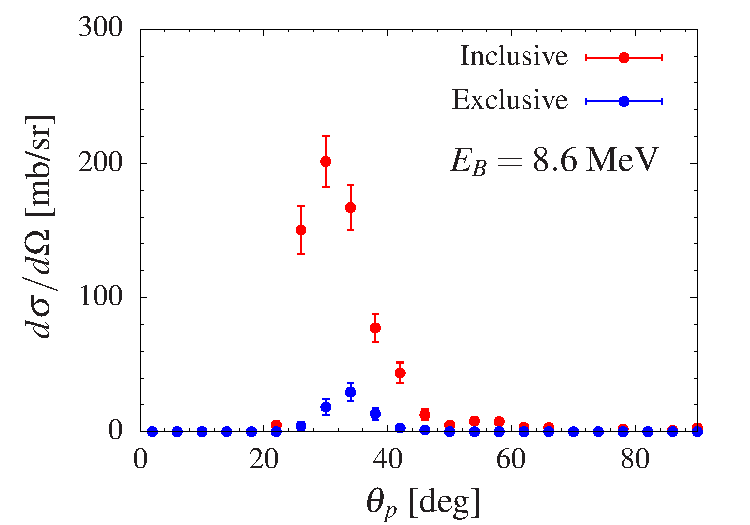
\includegraphics[width=0.49\textwidth]{ad_260.eps}\\
\includegraphics[width=0.49\textwidth]{ad_270.eps}
\includegraphics[width=0.49\textwidth]{ad_280.eps}\\
\includegraphics[width=0.49\textwidth]{ad_290.eps}
\includegraphics[width=0.49\textwidth]{ad_300.eps}\\
 \caption{\label{proton4}  Same as Fig.~\ref{proton1} but for a different energy range. }
 \end{figure}
 

\begin{figure}[!ht]
\centering
\includegraphics[width=0.49\textwidth]{enerd.eps}
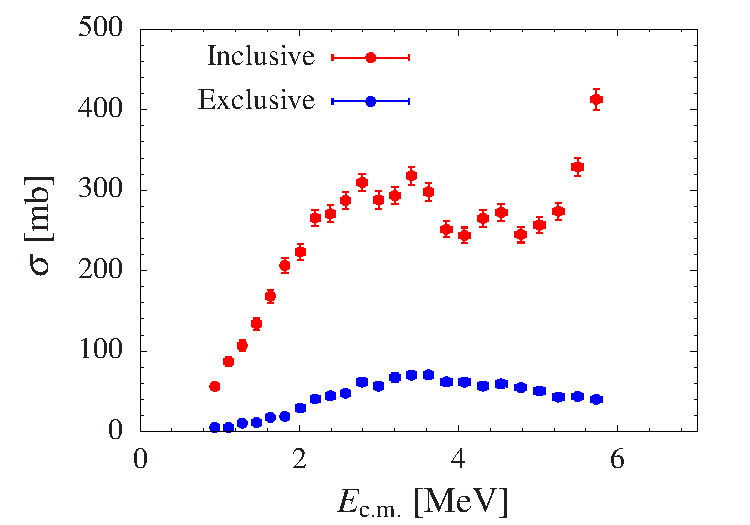
\includegraphics[width=0.49\textwidth]{enerdcm.eps}\\
 \caption{\label{ener}  Energy spectra of proton production at laboratory and center of mass energies. }
 \end{figure}
 
 
% \clearpage 
%%%%%====================================================================================
% \bibliography{bibliography}  % input bibliography
%%%%%====================================================================================




\end{document}

